\tikzset{%
	neuron missing/.style={
		draw=none, 
		scale=2,
		text height=0.1cm,
		execute at begin node=\color{black}$\vdots$
	},
}

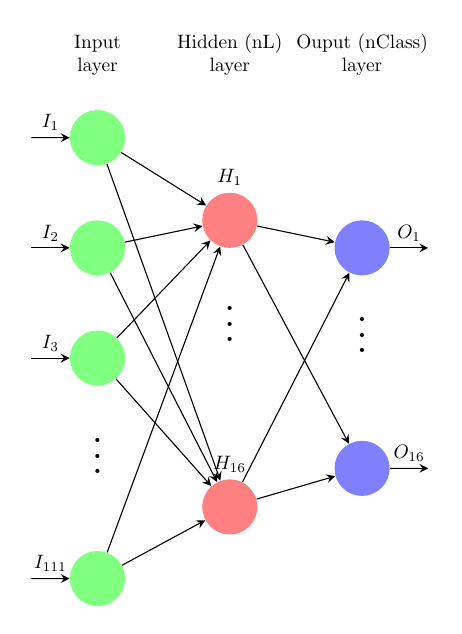
\begin{tikzpicture}[x=1.2cm, y=2cm, >=stealth,scale=.7, transform shape]
  % The grid
% \draw[step=0.5, gray!40, very thin] (-1,-3) grid (4,2);

%\node (A) at (.4, 1.8){$L_1$} ;
%\node[right,xshift=0.2cm] (B) at (3.5, 1.8) {$L_n$} ;
% arrows
%\draw[->, to path={-| (\tikztotarget)}] (A) edge (B) ;

%node[left, xshift=0.0cm, yshift=0.0cm,fill=orange!25,text width=1.3cm] {{\scriptsize Cell Type (LSTM, GRU)}};

%\draw[arrows=-latex]  (0,1.5) -- (-1.1,1)  node[left, xshift=0.0cm, yshift=0.05cm,fill=orange!25,text width=1.3cm] {{\scriptsize Cell Units (nU)}};

%\draw[arrows=-latex]  (0,1.5) -- (-1.1,2.2)  node[left, xshift=0.0cm, yshift=0.0cm,fill=orange!25,text width=1.3cm] {{\scriptsize Cell Type (LSTM, GRU)}};

\foreach \m/\l [count=\y] in {1,2,3}
{
	\node [circle,fill=green!50,minimum size=1cm] (input-\m) at (0,2.5-\y) {};
}
\foreach \m/\l [count=\y] in {4}
{
	\node [circle,fill=green!50,minimum size=1cm ] (input-\m) at (0,-2.5) {};
}

\node [neuron missing]  at (0,-1.5) {};


\foreach \m [count=\y] in {1}
\node [circle,fill=red!50,minimum size=1cm ] (hidden-\m) at (2,0.75) {};

\foreach \m [count=\y] in {2}
\node [circle,fill=red!50,minimum size=1cm ] (hidden-\m) at (2,-1.85) {};


\node [neuron missing]  at (2,-0.3) {};


\foreach \m [count=\y] in {1}
\node [circle,fill=blue!50,minimum size=1cm ] (output-\m) at (4,1.5-\y) {};

\foreach \m [count=\y] in {2}
\node [circle,fill=blue!50,minimum size=1cm ] (output-\m) at (4,-0.5-\y) {};

\node [neuron missing]  at (4,-0.4) {};


\foreach \l [count=\i] in {1,2,3,111}
\draw [<-] (input-\i) -- ++(-1,0)
node [above, midway] {$I_{\l}$};

\foreach \l [count=\i] in {1,16}
\node [above] at (hidden-\i.north) {$H_{\l}$};

\foreach \l [count=\i] in {1,16}
\draw [->] (output-\i) -- ++(1,0)
node [above, midway] {$O_{ \l}$};

\foreach \i in {1,...,4}
\foreach \j in {1,...,2}
\draw [->] (input-\i) -- (hidden-\j);

\foreach \i in {1,...,2}
\foreach \j in {1,...,2}
\draw [->] (hidden-\i) -- (output-\j);

\foreach \l [count=\x from 0] in {Input, Hidden (nL), Ouput (nClass)}
\node [align=center, above] at (\x*2,2) {\l \\ layer};

\end{tikzpicture}
